%----------------------------------------------------------------------------------------
%	PACKAGES AND THEMES
%----------------------------------------------------------------------------------------
\documentclass[aspectratio=169,xcolor=dvipsnames]{beamer}
\usetheme{Antibes}
\usecolortheme{beaver} 

\usepackage[utf8]{inputenc}
\usepackage{amsmath, amsfonts, amsthm, amscd, amssymb}
\usepackage{tikz} 
\usepackage[center]{caption}
\usepackage[vlined]{algorithm2e}
\usepackage{pgf,tikz}
\usepackage[french]{babel}
\usepackage{lmodern}
\usepackage[T1]{fontenc}
\usepackage{hyperref}
\usepackage{color}
\usepackage{graphicx} % Allows including images
\graphicspath{{Figures/}} %Setting the graphicspath
\usepackage{booktabs} % Allows the use of \toprule, \midrule and \bottomrule in tables
\usepackage{cancel}
\usepackage{animate}
\usepackage{array}
\usepackage{xcolor,colortbl}
\usepackage{subfigure}

% Pour les diagrams fait avec matcha
\usepackage{physics}
\usepackage{amsmath}
\usepackage{tikz}
\usepackage{mathdots}
\usepackage{yhmath}
\usepackage{cancel}
\usepackage{color}
\usepackage{siunitx}
\usepackage{array}
\usepackage{multirow}
\usepackage{amssymb}
\usepackage{gensymb}
\usepackage{tabularx}
\usepackage{extarrows}
\usepackage{booktabs}
\usetikzlibrary{fadings}
\usetikzlibrary{patterns}
\usetikzlibrary{shadows.blur}
\usetikzlibrary{shapes}

\usepackage{tikzit} % Pour les Tikz
\usepackage{tikzscale}
\input{Figures/sample.tikzstyles}
\usetikzlibrary{calc,patterns,angles,quotes}
%,scale=0.5, every node/.style={scale=0.5}


%\usepackage{physics}
%\usepackage{amsmath}
%\usepackage{mathdots}
%\usepackage{yhmath}
%\usepackage{siunitx}
%\usepackage{multirow}
%\usepackage{gensymb}
%\usepackage{tabularx}
%\usepackage{extarrows}
%\usetikzlibrary{fadings}
%\usetikzlibrary{patterns}
%\usetikzlibrary{shadows.blur}
%\usetikzlibrary{shapes}

\usepackage[%backend=biber,
style = ieee,
sorting=none
]{biblatex} %,bibstyle=ieeehttps://www.overleaf.com/project/624dc5f129c1767e8bb8de67
\addbibresource{biblio.bib}
\renewbibmacro*{date}{%
\iffieldundef{year}
{\bibstring{nodate}}
{\printdate}
}

% \usepackage{ulem}

\newcolumntype{a}{ >{\columncolor{blue}} c }

\setbeamertemplate{navigation symbols}{} % Remove the navigation symbols
\addtobeamertemplate{navigation symbols}{}{%
\usebeamerfont{footline}%
\usebeamercolor[fg]{footline}%
\hspace{1em}%
\insertframenumber/\inserttotalframenumber
}

\newcommand{\backupbegin}{
    \newcounter{framenumberappendix}
    \setcounter{framenumberappendix}{\value{framenumber}}
    }
    \newcommand{\backupend}{
        \addtocounter{framenumberappendix}{-\value{framenumber}}
        \addtocounter{framenumber}{\value{framenumberappendix}} 
        }
        
        \newcommand{\blue}[1]{\textcolor{blue!75}{#1}}
\newcommand{\green}[1]{\textcolor{teal!90}{#1}}
\newcommand{\red}[1]{\textcolor{red}{#1}}
\newcommand{\onlyred}[2]{\only<#1>{\red{#2}}}
\newcommand{\onlyblack}[2]{\only<#1>{#2}}
\newcommand{\rose}[1]{\textcolor{red!50}{#1}}

%\usepackage[bigfiles]{pdfbase}
\ExplSyntaxOn
\NewDocumentCommand\embedvideo{smm}{
  \group_begin:
  \leavevmode
  \tl_if_exist:cTF{file_\file_mdfive_hash:n{#3}}{
    \tl_set_eq:Nc\video{file_\file_mdfive_hash:n{#3}}
  }{
    \IfFileExists{#3}{}{\GenericError{}{File~`#3'~not~found}{}{}}
    \pbs_pdfobj:nnn{}{fstream}{{}{#3}}
    \pbs_pdfobj:nnn{}{dict}{
      /Type/Filespec/F~(#3)/UF~(#3)
      /EF~<</F~\pbs_pdflastobj:>>
    }
    \tl_set:Nx\video{\pbs_pdflastobj:}
    \tl_gset_eq:cN{file_\file_mdfive_hash:n{#3}}\video
  }
  %
  \pbs_pdfobj:nnn{}{dict}{
    /Type/RichMediaInstance/Subtype/Video
    /Asset~\video
    /Params~<</FlashVars (
      source=#3&
      skin=SkinOverAllNoFullNoCaption.swf&
      skinAutoHide=true&
      skinBackgroundColor=0x5F5F5F&
      skinBackgroundAlpha=0
    )>>
  }
  %
  \pbs_pdfobj:nnn{}{dict}{
    /Type/RichMediaConfiguration/Subtype/Video
    /Instances~[\pbs_pdflastobj:]
  }
  %
  \pbs_pdfobj:nnn{}{dict}{
    /Type/RichMediaContent
    /Assets~<<
      /Names~[(#3)~\video]
    >>
    /Configurations~[\pbs_pdflastobj:]
  }
  \tl_set:Nx\rmcontent{\pbs_pdflastobj:}
  %
  \pbs_pdfobj:nnn{}{dict}{
    /Activation~<<
      /Condition/\IfBooleanTF{#1}{PV}{XA}
      /Presentation~<</Style/Embedded>>
    >>
    /Deactivation~<</Condition/PI>>
  }
  %
  \hbox_set:Nn\l_tmpa_box{#2}
  \tl_set:Nx\l_box_wd_tl{\dim_use:N\box_wd:N\l_tmpa_box}
  \tl_set:Nx\l_box_ht_tl{\dim_use:N\box_ht:N\l_tmpa_box}
  \tl_set:Nx\l_box_dp_tl{\dim_use:N\box_dp:N\l_tmpa_box}
  \pbs_pdfxform:nnnnn{1}{1}{}{}{\l_tmpa_box}
  %
  \pbs_pdfannot:nnnn{\l_box_wd_tl}{\l_box_ht_tl}{\l_box_dp_tl}{
    /Subtype/RichMedia
    /BS~<</W~0/S/S>>
    /Contents~(embedded~video~file:#3)
    /NM~(rma:#3)
    /AP~<</N~\pbs_pdflastxform:>>
    /RichMediaSettings~\pbs_pdflastobj:
    /RichMediaContent~\rmcontent
  }
  \phantom{#2}
  \group_end:
}
\ExplSyntaxOff
%%%%%%%%%%%%%%%%%%%%%%%%%%%%%%%%%%%%%%%%%%%%%%%%%%%%%%%%%%%%%%%%%%%%%%%%%%%%%%

%----------------------------------------------------------------------------------------
%	TITLE PAGE
%----------------------------------------------------------------------------------------

% The title
\title[Simulation Numérique de \textit{l'Effet de Cheerios}]{Simulation Numérique de \textit{l'Effet de Cheerios}}
% \subtitle{Subtitle}

\author[Nous] {Baptiste BRAUN-DELVOYE\\\and Erdi ÇAN \\\and Projet en Calcul Scientifique LU2ME232}
\date{6 décembre 2022} % Date, can be changed to a custom date

\institute{Sorbonne Université, CMI Mécanique}

%----------------------------------------------------------------------------------------
%	PRESENTATION SLIDES
%----------------------------------------------------------------------------------------
\newcommand{\mycite}[1]{[\textcolor{blue!50}{#1}]}

\begin{document}
\usetikzlibrary{patterns,patterns.meta}
{
\setbeamertemplate{headline}{}
\begin{frame}
    \titlepage
    \centering
    
\includegraphics[scale=.2]{SORBONNE_FAC_SCIENCES_DEF_CMJN.png}
\end{frame}
}

\begin{frame}
    \frametitle{Sommaire}
    \tableofcontents
\end{frame}

\section{Introduction}
\begin{frame}{Introduction}% Probleme etudie
    \begin{center}
        % il faux que je compile ca dans mon windows je pense 
        %\embedvideo*{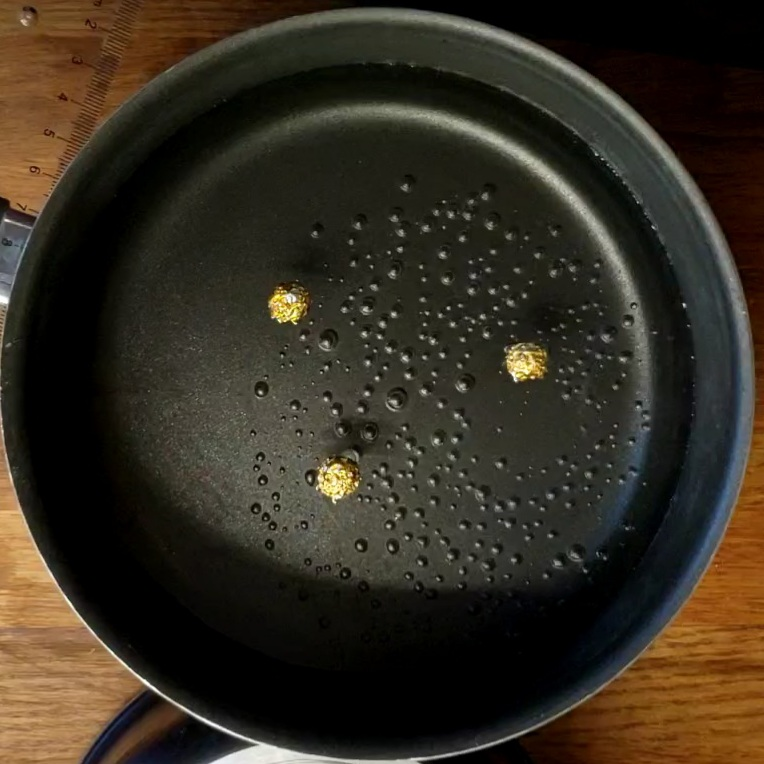
\includegraphics[width=0.4\textwidth]{image3AluFlottant.png}}{VideoDes3AluFlottant.mp4}
    \end{center}
\end{frame}

\section{Motivation}
\begin{frame}{Motivation}
    % Erdi aime trop la mécanique des fluides. Vous lui avez refusé son idée, on a pris cela à la place
    \begin{itemize}
        \item Nous aimons la mécanique des fluides
        \item Un projet trop ambitieux au départ\dots
        \item M. FULLANA nous a présenté l'Effet Cheerios
        \item Nous avons voulu simuler cet effet du mieux qu'on pouvait
    \end{itemize}
\end{frame}

\section{Modélisation de l'Effet de Cheerios}
% \begin{frame}{Modélisation de l'Effet de Cheerios\cite{vella_cheerios_2005}}
%     \begin{columns}
%         \begin{column}[]{0.3\textwidth}
%             \begin{figure}
%                 \centering
%                 \includegraphics[width=1.3\textwidth]{schema_geom_sphere_eau.tikz}
%                 \caption{\tiny{Géométrie d'une sphère reposant sur une interface liquide-gaz. La partie rayée représente le poids de liquide équivalent à la force de flottabilité du à la pression hydrostatique appuyant sur la sphère.}}
%                 \label{geom_sphere}
%             \end{figure}
%         \end{column}
%         \begin{column}[]{0.6\textwidth}
%             \[z_c^{'}\sin \phi_c = B\left(\frac{2D-1}{3}-\frac{1}{2}\cos \theta + \frac{1}{6} \cos^3 \theta\right) \equiv B\Sigma\]
%             Avec $B$ le nombre de Bond linéarisé et $D \equiv \rho_s / \rho_l$
%             \[E(l)=-2\pi\gamma R^2b^2\Sigma^2K_0\left(\frac{l}{L_c}\right)\]
%         \end{column}
%     \end{columns}
%     \begin{block}{Force d'interaction des objets flottants}
%         \[-\frac{dE}{dl} = F(l)=-2\pi\gamma RB^{5/2}\Sigma^2K_1\left(\frac{l}{l_c}\right)\]
%     \end{block}
% \end{frame}

\begin{frame}{Modélisation de l'Effet de Cheerios\cite{vella_cheerios_2005}}
    \centering
    \begin{figure}
        \centering
        \includegraphics[width=0.5\textwidth]{schema_geom_sphere_eau.tikz}
        \caption{Géométrie d'une sphère reposant sur une interface liquide-gaz.}
        \label{geom_sphere}
    \end{figure} 
    \[z_c^{'}\sin \phi_c = B\left(\frac{2D-1}{3}-\frac{1}{2}\cos \theta + \frac{1}{6} \cos^3 \theta\right) \equiv B\Sigma\]
    Avec $B$ le nombre de Bond linéarisé et $D \equiv \rho_s / \rho_l$
\end{frame}

\begin{frame}{Modélisation de l'Effet de Cheerios\cite{vella_cheerios_2005}}
    \[E(l)=-2\pi\gamma R^2b^2\Sigma^2K_0\left(\frac{l}{L_c}\right)\]
    \begin{block}{Force d'interaction des objets flottants}
        \[-\frac{dE}{dl} = F(l)=-2\pi\gamma RB^{5/2}\Sigma^2K_1\left(\frac{l}{l_c}\right)\]
    \end{block}

\end{frame}

\section{Méthodes Utilisées}
\subsection{Intégration de Verlet}
\begin{frame}{Méthodes Utilisées-\textit{Velocity Verlet}\cite{crivelli_stormer-verlet_2008}}
    \[\mathrm{DL}_3 \vb*{x}(t+\dd t)= \vb*{x}(t)+\vb*{v}(t)(\dd t)+\frac{\vb*{a}(t)}{2!}(\dd t)^2+o(\dd t^3)\]
    \[\sum  \vb*{F} = m\vb*{a} \Rightarrow \vb*{a} = \frac{\sum \vb*{F}}{m}\]
    \[\vb*{v}(t+\dd t) = \vb*{v}(t)+\frac{\vb*{a}(t)+\vb*{a}(t+\dd t)}{2}\dd t \]
    % \begin{block}{}
    % \end{block}
\end{frame}

\subsection{Détection des Collisions}
\begin{frame}{Méthodes Utilisées-Colisions Bords}
    \begin{columns}
        \begin{column}[]{0.5\textwidth}
            On peux décomposer le vecteur vitesse en:
            \[\vb*{v} = (\vb*{v}\cdot\vb*{n})\vb*{n} +(\vb*{v}\cdot\vb*{t})\vb*{t}\]
            \[\Rightarrow\vb*{v}^{'} = -(\vb*{v}\cdot\vb*{n})\vb*{n} + (\vb*{v}\cdot\vb*{t})\vb*{t}\]
        \end{column}
        \begin{column}[]{0.5\textwidth}
            \begin{figure}
                \centering
                \includegraphics[height = 0.7\textwidth]{rebond.tikz}
                \caption{Schéma d'un rebond d'un objet sur un bord}
            \end{figure}
        \end{column}
    \end{columns}
\end{frame}

\begin{frame}{Méthodes Utilisées-Colisions Objet-Objet}
    On détecte des collisions quand nos objets se chevauchent. Puis on applique la conservation du momentum.
    \begin{columns}
        \begin{column}[]{0.25\textwidth}
            \[\vb*{c} = \frac{\vb*{AB}}{||\vb*{AB}||}\]
            \[\vb*{v}_{rel} = \vb*{v}_A - \vb*{v}_B\]
            \[v_{col}=\vb*{v_{rel}}\cdot\vb*{c}\]
            % \[I = \frac{2v_{col}}{m_A + m_B}\]
            % \[\vb*{v}_A^{'} = \vb*{v}_A - Im_B\vb*{c}\]
            % \[\vb*{v}_B^{'} = \vb*{v}_B + Im_A\vb*{c}\]
        \end{column}
        \begin{column}[]{0.25\textwidth}
            % \[\vb*{c} = \frac{\vb*{AB}}{||\vb*{AB}||}\]
            % \[\vb*{v}_{rel} = \vb*{v}_A - \vb*{v}_B\]
            % \[v_{col}=\vb*{v_{rel}}\cdot\vb*{c}\]
            \[I = \frac{2v_{col}}{m_A + m_B}\]
            \[\vb*{v}_A^{'} = \vb*{v}_A - Im_B\vb*{c}\]
            \[\vb*{v}_B^{'} = \vb*{v}_B + Im_A\vb*{c}\]
        \end{column}
        \begin{column}[]{0.5\textwidth}
            \begin{figure}
                \centering
                \includegraphics[]{schema_collisions.tikz}
                \caption{Schéma d'une collision}
            \end{figure}
        \end{column}
    \end{columns}
\end{frame}


\section{Algorithme du code}
\begin{frame}{Algorithme du code}
    \begin{columns}
        \begin{column}[]{0.7\textwidth}
            \begin{itemize}
                \item[] Pour tout les pas de temps 
                {\setlength\itemindent{15pt} \item[] Pour tout les objets}
                {\setlength\itemindent{30pt} \item[] Pour tout les objets }
                {\setlength\itemindent{45pt} \item[] Si collision }
                {\setlength\itemindent{60pt} \item[] Applique collision}
                {\setlength\itemindent{45pt} \item[] Sinon}
                {\setlength\itemindent{60pt} \item[] Calcul force}
                {\setlength\itemindent{15pt} \item[] Met la force dans l'objet}
                \item[] Trouve nouvelles positions avec l'integration de Verlet 
                \item[] Écriture données à chaque itérations.
            \end{itemize}
        \end{column}
        \begin{column}[]{0.35\textwidth}
            \begin{block}{Complexité}
                \begin{itemize}
                    \item Complexité du temps de $O(NT\;n^2)$ 
                    \item Complexité de l'espace de $O(n)$
                \end{itemize}
                Avec n le nombre d'objets simulés
            \end{block}
        \end{column}
    \end{columns}
\end{frame}

\section{Résultats}
\begin{frame}{Résultats}
    Cest ici que on execute notre code?
\end{frame}

\section{Conclusion}
\begin{frame}{Conclusion}
    % Le projet peux avoir laire de etre facile mais comme nos forces ne sont pas conservatives et que on arette pas notre simulation quand on a des collisions et continue il ya pas mal de complications qui vienet
    \begin{itemize}
        \item Programme fonctionnel, mais pour qu'un diamètre en même temps.
        \item Résultats concluants par rapport à des expériences.
        \item Améliorations de nos compétences en programmation, calcul numérique et en mécanique du fluide.
    \end{itemize}
\end{frame}

\begin{frame}[allowframebreaks,noframenumbering]{Références}
    %\thispagestyle{empty}
    \nocite{*}
    %\addcontentsline{toc}{section}{Bibliographie}
    \printbibliography[title = Références]
\end{frame}

\end{document}


